The thesis examines the relative gain of a selfish miner in a peer-to-peer network similar to the original Bitcoin network.
The selfish miner is implemented by eclipsing a normal Bitcoin peer with a proxy.
The proxy then conducts selfish mining by withholding blocks created by the honest network and the eclipsed node.
The network and the containing nodes were realised by using \textit{Docker} and hence, virtualised on one single host.
Both approaches, the selfish proxy and the virtualised peer-to-peer network, are novel and are leaving many possibilities for improvement and research directions open.

\section{Selfish proxy}

The selfish proxy needs to receive information of new blocks as fast as possible to conduct selfish mining efficiently.
Currently, the proxy requests the whole block and all headers of blocks higher than its local best tip after hearing about a new block as described in chapter \ref{chap:receiving_blocks} and \ref{chap:sending_blocks}.
To successfully relay the block to the other side of the network, the selfish proxy needs to receive both messages entirely where especially the full block request is very time-consuming.
By using the compact block relay mechanism, the selfish proxy could speed up this whole communication.
The compact block relay mechanism shown in figure \ref{fig:compact_block_relay} is implemented in the Bitcoin reference implementation since late 2016 \cite{bitcoin13} and allows the node to broadcast blocks to its peers directly \cite{bip152}.
The difference to the normal block relay mechanism is that the node relays the block without any transactions.
To verify the block, the receiving node first checks which transactions are in the local mempool and asks afterwards with a specific request only for the missing transactions.
Compared to the traditional block relay mechanism where the node sends the full block containing all transactions, the compact block relay mechanism reduces the amount of data transferred and accelerates the block relay \cite{bip152, ozisik2017graphene}.
In the case of the selfish proxy, the update of the local chain could be executed right after the compact block is received.
Then, depending on the outcome of the selfish mining algorithm, the relevant blocks could be relayed using the compact block relay mechanism.
Compared to the currently used relay mechanism the whole communication flow would be reduced from six sent messages to two messages because during a simulation only empty blocks are created.
It is very likely that the compact block relay would improve the efficiency of the selfish mining strategy performed by the proxy, especially if at some later point also transactions are created during a simulation.
Then the transmission of the blocks is even more time consuming and increases the time needed by the proxy to relay blocks.

\begin{figure}[t]
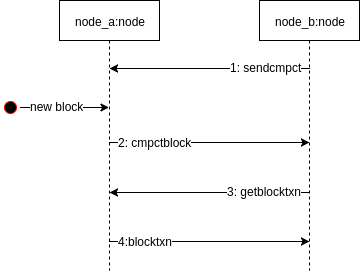
\includegraphics[width=8cm]{compact_block_relay}
\centering
\caption{Compact block relay mechanism \cite{bip152}}
\label{fig:compact_block_relay}
\end{figure}

Another direction of research consists of implementing the selfish mining strategies directly in the code executed by the nodes of the network.
For example, the publicly available reference implementation could be extended to implement selfish mining.
In the current setting, the selfish proxy adds an extra hop between the communication of the honest network and the eclipse node.
Hence, the proxy increases the latency of the eclipsed node significantly.
With the raised latency the position of the selfish miner during a block race is worsen resulting in a lower efficiency of the conducted selfish mining.
By implementing the selfish mining directly in the reference implementation, the extra hop would be removed, and the selfish miner now consisting only of one node would not have a lower latency compared to the honest network.
The downside of this approach would be that the reference implementation is altered which could cause unexpected side-effects.

Last but not least combining attacks with selfish mining provides a possible field of research.
The selfish miner could improve the profitability of the selfish mining by combining it with other attacks \cite{gervais2016security, sapirshtein2016optimal, nayak2016stubborn, gervais2015tampering}.
New insights and combinations could be tested by implementing and simulating the attacks directly in the simulation framework or selfish proxy.

\section{Simulation scenario}

Currently, no transactions are included in the simulation runs.
Thus, all blocks generated by the nodes are empty and consequently propagate faster in the network than a block with transactions.
A further research direction consists of including transactions in a simulation run to simulate the block propagation more realistically.
This could be either achieved by filling up the mempool with prepared transactions \todo[inline]{you mentioned that smb did this already, do you have a reference? didn't found anything. if not, we can leave it like this.} or by creating the transactions during the simulation run.
In the latter approach also the relaying of transactions would be simulated resulting in an even more realistic simulation.
Using this method the performance and reliability of the RPC-connections over TCP/IP needs to be considered.
The current implementation of the simulation framework has troubles to maintain the connection to the API of the nodes often resulting in \textit{broken pipe} errors.
At the moment these errors are recovered by simply reconnecting to the node which costs time.
Due to the lost time, the execution speed of the simulation needs to be lowered resulting in unsustainable long simulation durations.
Hence, to support the creation of transaction during a simulation run, the unreliability of the RPC-connections should be dissolved, or it should be considered to use the more performant Unix domain sockets.
The Unix domain sockets are providing their performance by bypassing the TCP/IP stack, and are likely to sustain the higher workload when adding transactions to a simulation scenario.
The capability to use Unix domain socket to communicate with the provided API by the nodes is planned for the next release of the reference implementation of Bitcoin \cite{bitcoinunixdomainsockets}.

Another compelling research area is the topology of the network and the nodes participating in the peer-to-peer network.
The network topology chosen in this thesis is just an abstract simplification of the real Bitcoin network.
The actual network changes continuously and contains multiple diverse nodes running different implementations of the Bitcoin protocol.
Hence, a better capturing of the actual topology of the Bitcoin peer-to-peer network containing dissimilar nodes could be an area of research.

\section{Mitigation}

The mitigation of selfish mining is also a possible future research direction.
The simulation framework and the proxy can be used to assess different proposed mitigation approaches \cite{eyal2014majority, billah2015one, solat2016zeroblock, zhang2017publish} against their impact on selfish mining.
Since the simulation framework uses the reference implementation a mitigation proposal like the uniform tie-breaking \cite{eyal2014majority} can be implemented directly in the actual code.
Hence, those mitigations can be tested quickly and under realistic circumstances providing accurate results.
